\documentclass[a4paper,12pt]{article}
\author{Baptiste Bainier et Thomas Jeantet}
\usepackage[french]{babel}
\usepackage{amsmath}
\usepackage{graphicx}
\usepackage{amsfonts}
\usepackage{pdflscape}
\usepackage[utf8]{inputenc}
\usepackage{float}



%Package
\usepackage[margin=1in]{geometry}
\usepackage{fancyhdr}
\usepackage{placeins}
\usepackage{listings}
\usepackage{color}
\usepackage[table,xcdraw]{xcolor}
\usepackage{ulem} %barrer du texte
\usepackage{cancel}% barrer dans une expression math (\cancel{})
\usepackage{pgf,tikz}
\usepackage{mathrsfs}
\usepackage{multirow}
%\usepackage{gensymb}
\usepackage{caption}
\usepackage{eurosym}% pour le symbole €



\usetikzlibrary{shapes.geometric, arrows}
\definecolor{qqqqff}{rgb}{0.,0.,1.}
%Configuration
\renewcommand*\contentsname{Sommaire}
\graphicspath{ {images/} }
%\renewcommand{\thesection}{\Roman{section}}
%\renewcommand{\thesubsection}{\Alph{subsection}}

\definecolor{codegreen}{rgb}{0,0.6,0}
\definecolor{codegray}{rgb}{0.5,0.5,0.5}
\definecolor{codepurple}{rgb}{0.58,0,0.82}
\definecolor{backcolour}{rgb}{0.95,0.95,0.92}
 
\lstdefinestyle{mystyle}{
    backgroundcolor=\color{backcolour},   
    commentstyle=\color{codegreen},
    keywordstyle=\color{magenta},
    numberstyle=\tiny\color{codegray},
    stringstyle=\color{codepurple},
    basicstyle=\footnotesize,
    breakatwhitespace=false,         
    breaklines=true,                 
    captionpos=b,                    
    keepspaces=true,                 
    numbers=left,                    
    numbersep=5pt,                  
    showspaces=false,                
    showstringspaces=false,
    showtabs=false,                  
    tabsize=2
}

\lstset{style=mystyle}
\renewcommand{\lstlistingname}{Script}


\pagestyle{fancy}
\fancyhf{}
\rhead{Baptiste Bainier et Thomas Jeantet}
\lhead{SY26 - Détection de formes par réseau de neurones}
\rfoot{Page \thepage}

\title{Projet SY26\\Détection de formes par réseau de neurones}
%\graphicspath{}
\begin{document}
\maketitle
\newpage
\newpage


\section*{Introduction}
  Le développement de notre réseau de neurones a été implémenté dans le cadre de l'UV SY26. L'objectif est de pouvoir détecter et différencier des formes apparaissant sur un écran. Il y a 6 formes différentes, chacunes de couleur différente. Il faut pouvoir les différencier quelle que soit leur taille et leur position sur l'écran.

  Le réseau doit être implémenté sur Raspberry Pi 3, et les images sont capturées par une Raspicam (v2).
\bigskip
\tableofcontents

\newpage
\section{Choix du framework}
  Dans un premier temps, nous avons du nous accorder sur le choix de l'environnement de travail. Deux options nous semblaient évidentes : 
  \begin{itemize}
    \item Programmer en C++ avec OpenCV
    \item Programmer à l'aide d'un framework
  \end{itemize}
  Nous avons étudié les avantages et les inconvénients de chaque méthode avant de commencer la programmation.
  
  \subsection{Utiliser OpenCV}
    La première option évidente aurait été de dévlopper nous même tout le programme en C++ à l'aide des librairies OpenCV. Il existe quelques librairies OpenCV permettant d'implémenter des réseaux de neurones, mais ces librairies n'utilisent que des couches MLP, ce qui est donc moins adapté que le framework que nous allons utiliser pour le traitement d'images.

    De plus, nous avons estimé que développer tout le code nous même en C++ avec OpenCV nous aurait pris énormément de temps, ce qui, couplé aux technologies restreintes de OpenCV (MLP uniquement), en fait une méthode peu intéressante.
  
  \subsection{Utiliser un framework}
    La deuxième solution est donc d'utiliser un framework. Cette méthode présente également quelques inconvénients : 
    \begin{itemize}
      \item Le temps de recherche des différents frameworks existants
      \item Le temps de formation au framework choisi
    \end{itemize}

    En effet, dans un premier temps nous avons dû nous renseigner sur les différents frameworks existants. Cette phase demande du temps, car il faut trouver tous les frameworks adaptés à notre sujet, puis trouver le plus adapté selon la documentation de chacun. Plusieurs frameworks se sont révélés intéressants, dont TensorFlow, PyTorch, ou Caffe que nous avons choisi.

    Utiliser un framework présente aussi des avantages :
    \begin{itemize}
      \item Le temps de déploiement du réseau
      \item La flexibilité du réseau
    \end{itemize}

    Le réseau est plus rapide à mettre en place, car il existe déjà de nombreuses "briques" programmées, ce qui nous permet d'avoir à seulement les adapter à notre cas. On dispose également d'un réseau plus flexible, car tous les éléments sont prévus pour que les paramètre puissent être changés facilement, ce qui nous évite de refaire tout le code pour un moindre changement dans le premier scénario.

    Nous avons donc choisi d'utiliser un framework, ce qui nous économise du temps de développement et nous permet de concentrer nos efforts sur l'optimisation du réseau de neurones plutôt que sur le développement de ce dernier. Nous avons choisi d'utiliser Caffe, car il semblait parfaitement adapté à notre projet (réseau de neurones pour la détection d'images), et de plus il est en grande partie rédigé en C++, qui est le langage que nous connaissons le mieux.

\newpage
\section{Prise en main de Caffe}
  Une fois le framework choisi, il faut le prendre en main. Il est nécessaire de comprendre son utilité et son fonctionnement avant de commencer à l'utiliser. Nous allons donc brièvement le présenter dans cette partie.
  
  \subsection{Du Caffe ?}
    \textit{"Caffe is a deep learning framework made with expression, speed, and modularity in mind."}
    Caffe est un framework qui permet de créer des réseaux de neurones sur-mesure, selon les besoins de l'utilisateur. Plusieurs "couches" sont déjà implémentées, il suffit ensuite de choisir quelles couches utiliser, et quels paramètres leur appliquer. Cette étape de design du modèle se fait facilement au travers d'un simple fichier type protobuf, contenant l'ordre et les paramètres de chaque couche. De nombreux modèles différents existent déjà, et sont mis à disposition par Caffe au travers de leur "zoo".

    L'utilisateur peut alors choisir d'utiliser une base de données existante, ou de créer sa propre database. De nombreux exemples sont déjà implémentés dans Caffe, ce qui nous permet de découvrir le fonctionnement du framework, mais aussi de nous inspirer de ces exemples pour créer notre réseau. Dans un premier temps, nous avons découvert le framework grâce à l'exemple du modèle LeNet, utilisé pour différencier les chiffres de la la base de données MNIST.
  
  \subsection{L'exemple MNIST}
    Caffe fournit un exemple très complet basé sur la classification de la base de données MNIST à l'aide du modèle LeNet. Nous nous sommes basés sur cet exemple pour comprendre le fonctionnement du framework. L'exemple MNIST nous montre donc comment définir un modèle grâce au fichier protobuf, et la lecture du code nous a permis de comprendre la prise en charge des bases de données par Caffe.
    L'exécution de cet exemple nous a également permis de vérifier la compilation et la bonne exécution de Caffe sur nos machines. C'est en se basant sur cet exemple que nous avons développé notre propre solution au problème de SY26.

\newpage
\section{Adaptation du framework}
  Après avoir pris en main le framework, et maîtrisé l'exemple MNIST, il faut adapter le framework pour qu'il puisse répondre à nos besoins. Nous avons choisi de nous baser sur l'exemple MNIST, qui permet de faire de la classification de 10 images différentes (les 10 chiffres). Nous pensons que ce modèle (LeNet) est relativement bien adapté à notre problème car la diversité des données en entrée est relativement similaire : nous avons 6 formes différentes à détecter (contre 10 pour LeNet), et nos formes ont toutes des contours différents, tout comme celles de la base de données MNIST. 

  De plus, il nous aurait fallu énormément de temps pour développer notre propre modèle, notamment à cause des temps d'apprentissages très longs sur nos machines, qui restreignent considérablement le nombre de modèles possibles à tester. Nous avons donc pensé qu'il était judicieux de se baser sur LeNet.
  
  \subsection{Data augmentation}
    La première différence entre l'exemple de la classification MNIST et notre classification est simplement la donnée d'entrée. Nous avons besoin de créer nos propres données d'apprentissage pour entrainer notre modèle. Pour créer une base de données suffisamment grande, nous avons décidé de faire de la "data augmentation". Nous avons pris plusieurs photos des images à identifier, que nous avons ensuite déformées de plusieurs manières afin de créer des données similaires mais différentes à apprendre à notre réseau.

    Nous avons essayé diverses transformations sur nos images d'origine :
    \begin{itemize}
      \item La rotation
      \item Le bruit gaussien
      \item Le bruit "SNP" (Salt an Pepper)
      \item La modification du contraste
      \item La modofcation de la luminosité
    \end{itemize}

    Ces transformations nous permettent donc de créer facilement quelques milliers d'images d'apprentissage à partir de quelques dizaines de photos. Nous avons essayé de prendre des photos dans différents lieux, et à différents moments de la journée, pour essayer d'avoir des données reflétant toutes les expositions de photos possibles.

    Nous avons testé beaucoup de valeurs différentes pour ces transformations, que nous avons changées en fonction de la réponse du réseau. Nous avons constaté qu'il n'est pas nécessaire de trop bruiter les images de la base de donnée, introduisant de la perte si le réseau ne peut pas reconnaitre la forme en entrée. Nous avons décidé de ne pas appliquer de rotation, le réseau LeNet n'étant à priori pas sensible à la rotation. De plus cette transformation implique l'ajout d'un bord noir sur chaque image.
    Nous avons décidé de ne pas utiliser le bruit SNP, ayant beaucoup trop d'influence sur les couleurs de l'image lorsque celles-ci sont trop petites. Le bruit gaussien a été gardé, mais à une amplitude limitée. Il reflète plus ou moins les différences de netteté sur l'image perçue par la raspicam (qui change selon l'exposition).
    Les modifications de contraste et de luminosité sont conservées, mais encore une fois à une amplitude limitée, car ces modifications sont susceptibles de générer des images inutilisables (trop noires ou trop blanches) si la luminosité d'origine est trop extrême. 

  \subsection{Création de database(s)}
    Une fois les images d'apprentissage générées, il faut générer les fichiers de bases de données. Deux fichiers sont créés : La database d'apprentissage,contenant toutes les images ainsi que les labels qui y sont associés, et la database de test, contenant d'autres photos (non augmentées). Ces fichiers sont écrits dans un format particulier, le format "LMDB". Nous avons récupéré et modifié un script Python qui permet de générer des bases de données lmdb à partir de nos images et de nos labels.
  
  \subsection{Personnalisation du net}
    Une fois la database créée, il faut adapter le modèle LeNet pour mieux correspondre à notre projet. Plus exactement, il faut modifier les hyperparamètres du modèle, car les couches que nous utilisons restent les même que celles de LeNet (Conv, Pool, Conv, Pool, Fully Connected MLP). La prochaine partie explicite les modifications que nous avons appliquées à ces hyperparamètres.

\newpage
\section{Evaluation des performances}
  Plusieurs paramètres influencent les performances d'un réseau, en plus de ses différentes couches. Nous allons détailler ici les paramètres que nous avons pu modifier au cours de ce projet, et leurs influences.
  \subsection{Le format des images}
    La formes des images que nous allions utiliser fut le premier paramètre que nous avons déterminé. 
    
    Tout d'abord, il faut choisir entre l'utilisation d'images couleur ou d'images en nuances de gris. Cependant, plus le nombre de canaux est grand, plus le temps d'apprentissage sera long. Nous avons tout de même choisi d'utiliser des images couleur, car chaque forme est associée à une couleur. 

    Il devrait être plus simple pour le réseau de repérer les différences entre chaque image.
    Ensuite il nous faut décider de la taille de chaque image. Une grande image impose beaucoup de calculs, il faut donc choisir une taille qui permette de distinguer les formes, quelle que soit leur taille. Nous avons choisi un format rectangulaire, de 96 par 54 pixel. Cette taille est un multiple de la résolution maximale de la caméra, 1920 par 1080, ce qui permet moins de pertes de qualité lors d'un changement de taille. Elle est également suffisamment grande pour discerner des petites formes.
    
  \subsection{Influence des images de la database}

  
  \subsection{Influence des hyperParamètres}
    L'apprentissage est une étape cruciale, possédant beaucoup de paramètres, dont nous allons voir l'influence.
    \subsubsection{Le learning rate et son évolution}
      Le learning rate est le paramètre le plus important lors de l'apprentissage; delui dépend la convergence ou non d'un réseau. Caffe nous permet de de faire varier ce learning rate en fonction du nombre d'itérations.

      Il n'y a pas de méthode particulière pour déterminer les bons paramètres, il faut lancer des apprentissages et observer la réponse du réseau. A force de tatônnements, nous sommes parvenus à une courbe de learning rate produisant une convergence assez rapide en phase de validation (environ 400 iterations), et permettant un loss bas, et une accuracy proche de 1.

    \subsubsection{Taille de batch}
      Un batch est le nombre d'image que l'on va fournir à notre réseau avant de changer les poids. Plus il y a d'images dans un batch, plus la descente de gradient sera précise, mais plus l'apprentissage est lent. De plus, si la taille de batch n'est pas un multiple du nombre d'images dans la base de donnée, on risque de favoriser l'apprentissage d'une classe au détriment d'une autre. 

      Selon le nombre d'images issus de la data augmentation, nous choisissons les batch size aux alentours de 60. Avecc cet ordre de grandeur, nous avons une vitesse d'apprentissage acceptable tout en convergeant.
    \subsubsection{Nombre de filtres}
      

\newpage
\section*{Conclusion}
  
  \subsection*{Améliorer notre réseau}
    Notre réseau peut encore être amélioré, et c'est ce que nous allons faire pendant les vacances pour avoir un modèle le mieux entraîné possible lors de notre présentation à la rentrée. Nous sommes actuellement en train de faire des tests avec différents hyperparamètre, seront joints en annexes quelques résultats de tests.
  
  \subsection*{Le Machine Learning}
    Cette UV et ce projet nous ont permis de découvrir le Machine Learning et ses applications. Nous avons appris le fonctionnement et la réalisation d'un réseau de neurones, et nous avons constaté la puissance de ces algorithmes, notamment dans le cadre de la classification d'images.
  
  \subsection*{Ce que le projet nous a apporté}
    Ce projet nous a permis de découvrir le Machine Learning, mais aussi de travailler avec un framework. Aucun d'entre nous n'avait travaillé avec des frameworks auparavant, et nous avons pu découvrir l'utilité d'utiliser ces environnements.

\newpage
\section*{Annexes}
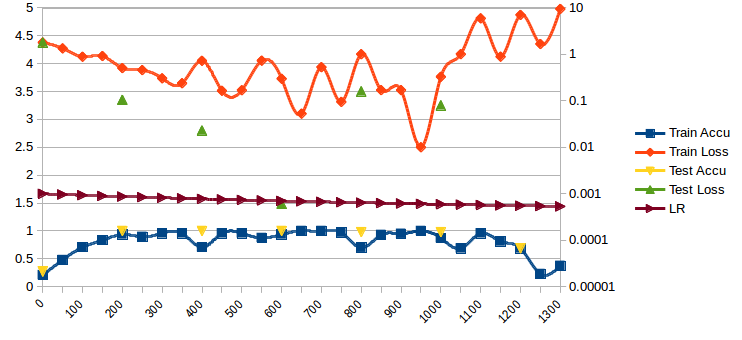
\includegraphics[keepaspectratio=true,width=430]{graphs/graph1.png}
    \caption{ta soeur}

\end{document}
